% Header and Footer
\pagestyle{fancy}
%\fancyfoot[L]{}
\fancyfoot[C]{By: \myName}
\fancyfoot[R]{\thepage}
\renewcommand{\headrulewidth}{0.4pt}
\renewcommand{\footrulewidth}{2pt}

\section{UQ Subjects} %\label{sec_introduction}
This chapter goes through the UQ courses that was undertaken from 2016-2019. The format will be as follows, for each section, where possible:
\begin{enumerate}
  \item Lecture notes (Use ``LEC\#\#: TITLE HERE'' for each heading)
  \item Tutorial questions (Use ``TUT\#\#: TITLE HERE'' for each heading)
  \item Summary of all equations used (Use ``EQU\#\#: TITLE HERE'' for each heading)
  \item References \& other helping material (Use ``REF\#\#: TITLE HERE'' for each heading)
  \item Australian Standards (Use ``STD\#\#: TITLE HERE'' for each heading)
\end{enumerate}

In terms of text colour and highlights, the format will be as follows where possible:
\begin{enumerate}
  \item Black = normal text
  \item \textcolor{red}{Red = Important}
  \item \textcolor{blue}{Blue = References}
  \item \textcolor{green}{Green = Key Takeaways}
\end{enumerate}

% TOPIC: CODING
\subsection{CSSE2002 - Java Language}
\clearpage

\subsection{CSSE2010 - Embedded Programming}
\clearpage

\subsection{CSSE2310 - C Language}
\clearpage

\subsection{CSSE3010 - Advanced Embedded}
\clearpage

% TOPIC: MATHEMATICS
\subsection{MATH1051 - Linear Calculus}
\clearpage

\subsection{MATH2001 - Advanced Calculus}
\clearpage

\subsection{MATH2010 - Partial Differential Equations}
\clearpage

\subsection{STAT2202 - Advanced Statistics}
\clearpage

% TOPIC: ELECTRICAL KNOWLEDGE
\subsection{ELEC2003 - Electronics \& Circuits Pt.1}
\clearpage

\subsection{ELEC2004 - Electronics \& Circuits Pt.2}
\subsubsection{LEC01: Capacitors and Inductors, RL and RC Circuits}
\textsc{\large Capacitors}\\
Capacitors and inductors are linear circuit elements that can store electrical energy. The ideal capacitor stores energy in the form of \textbf{charge}.

\begin{align} \label{eq_ELEC2004_capacitance}
  C &= \frac{\epsilon A}{d}
\end{align}
Where:
\begin{itemize}
  \item C = capacitance in Farads ($F$)
  \item A = conductor plates area (both top and bottom) ($mm^2$)
  \item $\epsilon$ = dielectric of permitivity (constant)
  \item d = plate separation distance ($m$)
\end{itemize}

\begin{align} \label{eq_ELEC2004_charge}
  Q &= CV
\end{align}
Where:
\begin{itemize}
  \item Q = stored charge
  \item C = capacitance ($F$)
  \item V = applied voltage ($V$)
\end{itemize}

In DC, a capacitor is effectively an open circuit; when a steady voltage is applied. \textcolor{red}{When the voltage changes, the stored charge changes also as per equation \eqref{eq_ELEC2004_charge} by taking the derivative.} Thus,
\begin{align}
  i(t) &= \frac{dq(t)}{dt} = C \frac{dv(t)}{dt}
\end{align}
\textcolor{green}{KEY TAKEAWAY: Change in voltage induces a current because there are charges moving. This electrical energy is stored in ``capacitance'' in the form of an electric field.}\\
\\
Energy storage in capacitors is calculated by integrating the instantaneous power $P(t)$. Thus,
\begin{align}
  P(t) &= v(t)i(t) = Cv(t)\frac{dv(t)}{dt}
\end{align}
Integrating the instanteous power:
\begin{align}
  W(t) = \frac{1}{2}Cv^2(t)
\end{align}

Capacitors can be combined in series and in parallel to yield a single equivalent capacitance. Note: the behaviour of equivalent capacitance is the opposite of resistors. Series:
\begin{align}
  C_{EQ} &= \frac{1}{\frac{1}{C_1} + \frac{1}{C_2} + \frac{1}{C_3} ...}
\end{align}
Parallel:
\begin{align}
  C_{EQ} &= C_1 + C_2 + C_3 ...
\end{align}

\textsc{\large Inductors}\\
The ideal inductor stores energy in an \textbf{induced magnetic field}.

\begin{align}
  \phi &= LI
\end{align}
Where:
\begin{itemize}
  \item $\phi$ = induced magnetic flux
  \item L = inductance in Henrys ($H$)
  \item I = applied current ($A$)
\end{itemize}

In DC, an inductor is effectively a short circuit (i.e. a wire with no resistance). \textcolor{red}{When the current changes, the induced field also changes.} Thus,

\begin{align}
  v(t) &= \frac{d\phi(t)}{dt} = L \frac{di(t)}{dt}
\end{align}

\textcolor{green}{KEY TAKEAWAY: The rate of change in magnetic flux induces a voltage. Thus, alternating current (AC) induces a change in magnetic field and thus produces a voltage. Inductance is the tendency of an electrical conductor to oppose a change in the electric current flowing through it.}\\
\\
Energy storage in inductors is calculated by integrating the instantaneous power $P(t)$. Thus,
\begin{align}
  P(t) &= v(t)i(t) = Li(t)\frac{di(t)}{dt}
\end{align}
Integrating the instanteous power:
\begin{align}
  W(t) = \frac{1}{2}Li^2(t)
\end{align}

Inductors can be combined in series and in parallel to yield a single equivalent inductance. Note: the behaviour of equivalent inductance is the same as resistors. Series:
\begin{align}
  L_{EQ} &= L_1 + L_2 + L_3 ...
\end{align}
Parallel:
\begin{align}
  L_{EQ} &= \frac{1}{\frac{1}{L_1} + \frac{1}{L_2} + \frac{1}{L_3} ...}
\end{align}

Other topics found:
\begin{itemize}
  \item Solving RC Circuits \& Forced responses \& Transient analysis
  \item Approaches to solve circuits
  \item Class exercises
\end{itemize}
\clearpage

\subsubsection{LEC02: Nodal \& Mesh Analysis and Network Theorems}
\textsc{\large The Basics}\\
These are the fundamental electrical basics:
\begin{itemize}
  \item \textcolor{green}{$V = IR$ (Ohm's Law)}
  \item \textcolor{green}{$P = VI = \frac{V^2}{R} = I^2R$}
  \item \textcolor{green}{Kirchhoff's current law (KCL): Sum of currents into a node = 0}
  \item \textcolor{green}{Kirchhoff's voltage law (KVL): Sum of voltages around a loop = 0}
  \item \textcolor{green}{Series and parallel circuits (voltage and current dividers)}
\end{itemize}

\textsc{\large Mesh and Node Analysis}\\
\begin{itemize}
  \item Nodal analysis: Set voltages at each node as the unknown variables, apply KCL. Note: Currents going into the node are positive, and currents going out of the node are negative. Use KCL when the source is a current source.
  \item Mesh analysis: set the current through each branch as the unknown variables, apply KVL;  Note: choose a direction for a loop and stick to that direction for all loops. Voltages going from negative to positive (e.g. Voltage Sources) are positive and voltages going from positive to negative (e.g. resistors) are impedances. Use KVL when the source is a voltage source.
\end{itemize}
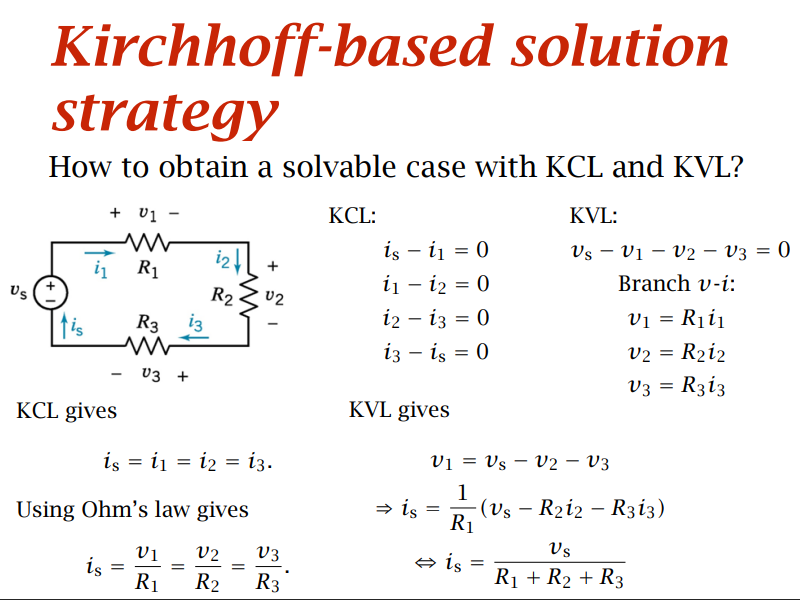
\includegraphics[width=\textwidth]{/02_UqSubjects/kirchhoffs}


\clearpage

\subsection{ELEC3100 - Advanced Electrical Theory}
\clearpage

\subsection{ELEC3300 - Motors \& Electrical Energy}
\clearpage

\subsection{ELEC3400 - Amplifiers \& Electronics}
\clearpage

\subsection{ELEC4300 - Power System Analysis}
\clearpage

\subsection{ELEC4302 - Power System Protection}
\clearpage

\subsection{ELEC4620 - Signal Processing}
\clearpage

\subsection{ELEC4630 - Image Processing}
\clearpage

% TOPIC: PROJECT MANAGEMENT
\subsection{ENGG4800 - Project Management}
\clearpage

% TOPIC: CONTROLS
\subsection{METR4201 - Control System Analysis}
\clearpage





\begin{comment}
\begin{figure}[!htpb]
    \vspace{-3mm}
  \centering
    {
        \includegraphics[width=0.8\textwidth]{figures/asset_overview.png}
    }
    \caption{Sample Asset Management User Interface Display: Asset Overview Screen}
    \label{fig:ui_mockup_overview}
    \vspace{-1mm}
\end{figure}

\begin{figure}[!htpb]
    \vspace{-3mm}
  \centering
  	{
        \includegraphics[width=0.9\textwidth]{figures/asset_specific.png}
    }
    \caption{Sample Asset Management User Interface Display: Asset Lookup Screen}
    \label{fig:ui_mockup_jackHammer}
    \vspace{-1mm}
\end{figure}

Megacorp’s culture is to diversify their knowledge base and keep an open mind for new projects.  The project will align with Megacorp’s by giving employees the opportunity to grow in their technical knowledge, leadership and teamwork. The proposed asset management system will be largely targeted to construction and mining companies. This leverages a customer base, most of whom, may already be Megacorp customers. The project stakeholders include Megacorp and construction company clientele.\\

With more than 70,000 construction companies listed in Australia, the potential market size is 3500 clients if 5\% penetration is assumed~\cite{RefI2}. Table~\ref{tab_competitors} below gives an overview of the features of the proposed product compared to the closest competitors. Several services and features of the proposed product will address deficiencies of the existing competitors and set Megacorp ahead of the competition.

\begin{table}[!htpb]
    \vspace{-1mm}
  \centering
  	{
        \includegraphics[width=0.8\textwidth]{figures/competitors.png}
    }
    \caption{Asset Management Product Competitor Comparison~\cite{RefI3, RefI4, RefI5, RefI6, RefI7} (Key: green = product capability, yellow = product deficiency)}
    \label{tab_competitors}
    \vspace{-1mm}
\end{table}
\end{comment}
